\documentclass{beamer}
\usepackage{feynmp} % setup feynmp
\DeclareGraphicsRule{*}{mps}{*}{}
\usepackage{tikz}

% theme and general look
\usetheme{Rochester}
\usecolortheme{seahorse}

\setbeameroption{show notes}

% title information
\title[Muon Pair Production]{Muon Pair Production from Electron Positron Annihilation}
\author{L.~Siemens}


\begin{document}
\begin{fmffile}{presentation_mp} % begin feynmp environment


\begin{frame}
    \titlepage
    %\note{\tableofcontents}
    \note[item]{Give brief introduction}
    \note{For my project I choose the computational project focusing on muon pair production. I will briefly introduce the mathematical methods used, outline the basic equations and simulation procedure, and present the result of the simulation.\vfill}
\end{frame}


\section{Setup}
\subsection{Monte Carlo methods}
\begin{frame}{Mathematical Methods: Monte Carlo Integration}
%    \begin{columns}
%        \column{0.5\textwidth}
        Average of a function $<f(x)> = \frac{1}{b-a}\int_a^b f(x)dx$

        \begin{block}{Monte Carlo Integration}
            $\int_a^b f(x)dx = (b-a)<f(x)>$
        \end{block}
        \note[item]{Simplest version of Monte Carlo integration derived directly from the definition of the average of the function on a domain}

        \begin{block}{Estimated Error}
            \begin{itemize}
                \item $N$ uniform random points
                \item $\sigma_{error} \propto 1/\sqrt{N}$
            \end{itemize}
        \end{block}
        \note[item]{The error in the integral estimate is proportional to the standard error of the mean.}

        \note[item]{Notice that the error is independent of the dimension of the integral.}

        \note{In its simplest form Monte Carlo integration is derived directly from the definition of the average of a function over some domain. So the value of an integral can be estimated given you have an estimate of this average. If you compute the average by sampling the function at random points in the domain, then the error in the estimate will be the standard error of the mean multiplied by the size of the domain. Note that this can be generalized to higher dimensions but the relationship between the number of samples and the error remains the same.\vfill}

%        \column{0.5\textwidth}
%        \includegraphics[height=0.5\textheight]{./Figures/angular.png}
%    \end{columns}
\end{frame}


\begin{frame}{Mathematical Methods: Monte Carlo Sampling}{Rejection Sampling}
%    \begin{columns}
%        \column{0.5\textwidth}
		\begin{block}{Rejection Sampling}
			Reproduce the distribution $f(x)$ on the domain $[a, b]$
			\note[item]{Method for reproducing arbitrary distributions.}
            \begin{enumerate}
                \item Sample the domain $[a, b] \times [0, 1]$ labeling points $(x_i, v_i)$
                \item Remove any sample with $v_i > f(x_i)/f_{max}$
            \end{enumerate}
            \note[item]{Note that the maximum of the function n the domain must be known beforehand.}
        \end{block}

        \note{Rejection sampling, a type of Monte Carlo sampling, is used to produce random samples from a specified distribution. The procedure consists of sampling a point in the domain and a value between zero and one, from uniform distributions. This sample will be rejected, if the random value from the unit interval exceeded the ratio of the value of the function at the sampled point to the maximum of the the function on the domain. The samples which have not been rejected will reproduce the desired statistical distribution, but to use this method the maximum of the function over the domain must be known beforehand.\vfill}
%        \column{0.5\textwidth}
%        \includegraphics[width=\textwidth]{./Figures/angular.png}
%    \end{columns}
\end{frame}


\subsection{Equations and differential cross section}
\begin{frame}{Muon Pair Production: $e^+ + e^- \rightarrow \mu^+ + \mu^-$}
    \begin{columns}
        \column{0.60\textwidth}
        \begin{block}{Expected number of events}
            $N_{exp} = L_{int} \cdot \sigma_{tot}$
        \end{block}
        \note[item]{Expected number of events from time integrated luminosity and the total cross section}

		\begin{block}{4-Momentums}
			Using the relativistic limit in the center of momentum frame
            \begin{itemize}
                \item $p_1^{\mu} = (E, 0, 0, E)^{\mu}$
                \item $p_3^{\mu} = (E, E\sin(\theta), 0, E\cos(\theta))^{\mu}$
            \end{itemize}
        \end{block}
        \note[item]{Note that the angle $\theta$ is the angle of the out going muon relative to the incoming electron.}

        \note{Moving on to the physics of the simulation. As I said before I am simulating muon pair production. Recall that the total number of expected scattering events is given by the time integrated luminosity and total scattering cross section. The calculations used for the differential cross section contains contributions from both the photon and Z boson Feynman diagrams. Also, I should note that the angle theta corresponds to the angle between the out going muon and the incoming electron.\vfill}

        \column{0.40\textwidth}
        \begin{fmfgraph*}(100, 80)
            \fmfleft{i2,i1}
            \fmfright{o4,o3}
            \fmf{fermion}{i1,v1,i2}
            \fmf{fermion}{o4,v2,o3}
            \fmf{photon, label=$\gamma,,Z^0$}{v1,v2}
            \fmflabel{$e$}{i2}
            \fmflabel{$\mu$}{o4}
            % Momentum arrows
            \fmfcmd{%
                vardef normal (expr p, mag) = 
                    (1, 0)
                    rotated (90 + angle direction 0.5*length(p) of p)
                    scaled mag
                enddef;
                % draw momentum arrow on left side of ray
                style_def marrowl expr p =
                    drawarrow subpath (1/4, 3/4) of p
                    shifted normal (p, 6)
                    withpen pencircle scaled 0.4;
                enddef;
                % draw momentum arrow on right side of ray
                style_def marrowr expr p =
                    drawarrow subpath (1/4, 3/4) of p
                    shifted normal (p, -6)
                    withpen pencircle scaled 0.4;
                enddef;}
            \fmf{marrowr, label=$p_1$, tension=0}{i1,v1}
            \fmf{marrowr, label=$p_3$, tension=0}{v2,o3}
        \end{fmfgraph*}

        \begin{figure}
            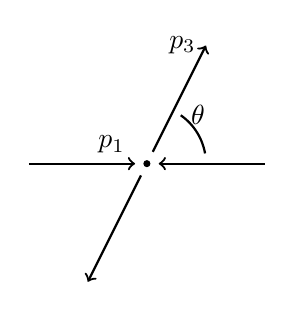
\begin{tikzpicture}[scale=1.5]
                \draw [thick,->] (-1,0) -- (-0.1,0) node[above left] {$p_1$};
                \draw [thick,<-] (0.1,0) -- (1,0);
                \draw [thick,->] (0.05,0.1) -- (0.5,1) node[left] {$p_3$};
                \draw [thick,domain=10:55] plot ({0.5*cos(\x)}, {0.5*sin(\x)}) node[right] {$\theta$};
                \draw [thick,<-] (-0.5,-1) -- (-0.05,-0.1);
                \draw [fill] (0,0) circle [radius=0.025];
            \end{tikzpicture}
        \end{figure}
    \end{columns}
\end{frame}


\begin{frame}{Differential Cross Section}
    Diagram amplitudes: $A_{\gamma}$, $A_{Z}$

    \begin{block}{$Z^0$ Vertex factor}
        \begin{itemize}
            \item $\frac{-ig_z}{2}\gamma^{\mu}(c_V^f - c_A^f\gamma^5)$
            \item For electorns and muons: $c_V^f = -\frac{1}{2} + 2\sin^2\theta_w$, $c_A^f = -\frac{1}{2}$
            \item $g_z = \frac{g_e}{\sin\theta_w\cos\theta_w}$
        \end{itemize}
        \note[item]{The term $\gamma^5$ in the vertex factor leads to the antisymmetric factors of $\cos(\theta)$ in the spin averaged amplitude squared.}
    \end{block}

    \begin{alertblock}{Angular dependence of $<|A|^2>$}
        $<|A|^2> = <|A_{\gamma}|^2> + <|A_{Z}|^2> + <A_{\gamma}A_Z^* + A_ZA_{\gamma}^*>$
        \begin{itemize}
            \item $<|A_{\gamma}|^2> \propto 1 + \cos^2(\theta)$
            \item $<|A_Z|^2> \propto 1 + \cos^2(\theta) + a\cos(\theta)$
            \item $<A_{\gamma}A_{Z}^* + A_{Z}A_{\gamma}^*> \propto 1 + \cos^2(\theta) + b\cos(\theta)$
        \end{itemize}
        \note[item]{All three terms have different dependence on the energy.}
        \note[item]{The factors $a$ and $b$ have different dependence on the vector-axial couplings}
    \end{alertblock}

    \note{Unlike the scattering amplitude due to the photon, the amplitude $A_Z$ contains factors of $\gamma^5$ and it is a function of a parameter called the weak mixing angle, $\theta_w$. Note the weak mixing angle defines the relationship between the electromagnetic and weak force. When applying Casimir's trick these factors of $\gamma^5$, in the pure Z boson component and in the cross terms, lead to factors of $\cos(\theta)$ which is antisymmetric about the centre of the interval $[0, \pi]$. Note that the photon term, the Z boson term and cross terms each have a different functional dependence on the energy, and the antisymmetric components of the Z boson term and the cross terms carry different factors of the weak mixing angle.\vfill}
\end{frame}


\subsection{Simulation Outline}
\begin{frame}{Monte Carlo Simulation}
    \begin{block}{Procedure}
        \begin{enumerate}
            \item Estimate $\sigma_{tot}$
            \note[item]{Calculate the maximum of $\frac{d\sigma}{d\Omega}\sin(\theta)$ using the samples of the function takin in the Monte Carlo integration}

            \item Expected number of events $N_{avg}$
    %        \item Sample from Poisson distribution with mean $N_{avg}$
            \item Sample one value, $N \sim Poisson(N_{avg})$
            \note[item]{Note, using the Poisson distribution is only necessary if the number of expected events $N_{avg}$ is small. TODO rephrase}

            \item Generate $N$ samples, $\theta \sim \frac{d\sigma}{d\Omega}d\Omega$
            \note[item]{This simulates muon pair production events at a fixed energy with out accounting for effects in the detector . . .}
            \item Calculate $p_3^{\mu}$
        \end{enumerate}
        \note[item]{With multiple runs at fixed integrated luminosity at a variety of energies. TODO finish}
    \end{block}

    \note{The procedure I used for simulating scattering events is as follows. \textbf{First}, for a given energy estimate the total cross section using Monte Carlo integration, and using the samples of the distribution generated for the integral, find the maximum of the differential cross section. \textbf{Second}, find the expected number of scattering events given the integrated luminosity and the total cross section. \textbf{Third}, get a random sample, labelled $N$, from a Poisson distribution with mean equal to the expected number of events, note that this step is only relevant when the expected number of scattering events is small, of order 10. \textbf{Fourth}, use rejection sampling to generate $N$ random angles from the distribution determined by the differential cross section. \textbf{Finally}, use the sampled angles and the energy to compute and record the 4-momentum of the muon. Repeating this procedure while keeping the integrated luminosity constant but varying the energy can be used to probe the energy dependence of the cross section.\vfill}
\end{frame}


\section{The Data}
\subsection{Angular and Energy Distributions}
\begin{frame}{Angular Distribution}
    \centering
    \includegraphics[height=0.8\textheight]{./Figures/angular_distribution.png}
    \note[item]{Note the symmetry and asymmetry of the differnt components}
    \begin{itemize}
        \item Integrated luminosity at LEP (year 2000): $2.33\times10^{-11}$ $1/mb$ 
        \note[item]{Expected results given the total luminosity of LEP for the year of 2000}
        \note[item]{On close inspection the contribution from Z bosons has a slight asymmetry}
    \end{itemize}

    \note{The first data set was generated with the integrated luminosity of the entirety of the year 2000 at the LEP, using a beam energy of 40 GeV. It should be noted that while the Z boson component looks symmetric at this scale, on close inspection it has a slight asymmetry. Also since the three components have different functional dependence on the energy the overall angular distribution will change as a function of energy and with varying degrees of asymmetry.}
\end{frame}


\begin{frame}{Cross Section vs Energy}
    \includegraphics[width=\textwidth]{./Figures/energy_distribution.png}
    \note[item]{fitting models to find the mass and decay width of the $Z^0$ boson.}
    \note[item]{The theoretical curves shows the trend but to match the data it has to be binned.}
    \begin{itemize}
        \item Integrated luminosity at LEP (year 2000): $2.33\times10^{-11}$ $1/mb$
        \item Energies upto the maximum beam energy of LEP: $[10m_{\mu}, 104.5GeV]$
    \end{itemize}
    \note{The second run uses the same total integrated luminosity but split across multiple beam energies ranging from ten times the rest energy of the muon to the maximum beam energy of the LEP in the year 2000. On the left you can see the results from the simulation compared to the expected number of events, and that is further broken down into the photon and Z boson contributions. Also notice that while the simulated events follow the same general trend as the analytic result, in the regions where the expected number of events changes rapidly with a single bin the discrepancy is significant. But this is to be expected as a side effect of binning the simulated data, averaging the analytic result over each bin like in the graph on the right now produces a fair comparison and now there are no significant outliers.}
\end{frame}


\subsection{Forward Backward Asymmetry}
\begin{frame}{Forward Backward Asymmetry}
    \centering
    \includegraphics[width=0.5\textwidth]{./Figures/AFB.png}
    \note[item]{At large energy the majority of muons are traveling in the same direction as the original electrons.}
    \note[item]{This mesurement can be used to determin the weak mixing angle by finding the best fit model given a range of parameters.}
    \begin{block}{Asymmetry}
        \begin{itemize}
            \item $A_{FB} = \frac{N_F - N_B}{N_F + N_B}$
            \item $N_F$, number of events with $0 < \theta < \pi/2$
            \item $N_B$, number of events with $\pi/2  < \theta < \pi$
        \end{itemize}
    \end{block}
    \note{Finally, considering the asymmetry in the angular distribution. The graph shown uses the same data set as in the previous slide, but for each energy bin the events have been separated into two groups, depending if the muon is moving forward along the direction in which the electron was moving. Using this the overall asymmetry in the muon distribution can be characterized. Notice, that as expected since QED does not violate parity, at low energy where the interaction is mediated by the photon the forward-backward asymmetry is approaching zero. Provided that the mass of the W boson has been measured in an anologus experement, measuring the mass of the Z boson provides one way to measure the weak mixing angle since the weak mixing angle is related to the ratio of the masses of Z and W bosons. Alternativly measurements of the forward backward asymmetry can be used to measure the weak mixing angle by finding a best fit out of models with different values for the weak mixing angle.}
\end{frame}

\end{fmffile}
\end{document}
